\titledquestion{Floyd-Warshall algorithm}
\begin{parts}
    \part[4] Consider the following pseudo-code of the Floyd-Warshall algorithm. Assume $w_{ij}=\infty$ where there is no edge between vertex $i$ and vertex $j$, and assume $w_{ii}=0$ for every vertex $i$.
\begin{figure}[htbp]
    \centering
    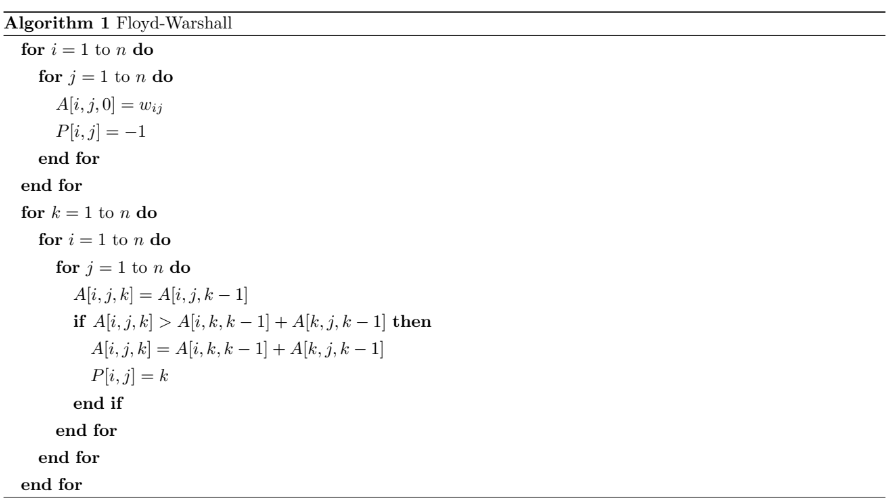
\includegraphics[width=1\linewidth]{fig/floyd-warshall.png}
\end{figure}
Assume matrix $P$, the output of the above algorithm, is given. Design an algorithm for finding the shortest path from $u$ to $v$ by using matrix $P$. You can show your algorithm with natural language or pseudo-code.
we can use the funcion $solution(u, v)$ to get the path from $u$ to $v$.
\begin{algorithm}[H]
    \begin{algorithmic}[1]
        \Function {solution}{$u$, $v$}
        \State path = []
        \If {$u == v$}
            \State path.push_back($u$)
            \State \Return path
        \EndIf
        \State path.push_back($u$)
        \State getpath($u, v, path$)
        \State path.push_back($v$)
        \State \Return path
        \EndFunction
    \end{algorithmic}
\end{algorithm}
to finish the getpath function above, we need to define a new function $getpath(u, v, path)$
\begin{algorithm}[H]
    \begin{algorithmic}[1]
        \Function {getpath}{$u, v, path$}
        \State $k = p[u, v]$
        \If {$k == -1$} 
            \State \Return 
        \EndIf
        \State getpath($u, k, path$)
        \State path.push_back($k$)
        \State getpath($k, v, path$)
        \EndFunction
    \end{algorithmic}
\end{algorithm}


\newpage

	\part[6] 
	Consider the following implementation of the Floyd-Warshall algorithm. Assume $w_{ij}=\infty$ where there is no edge between vertex $i$ and vertex $j$, and assume $w_{ii}=0$ for every vertex $i$. Add some codes in the blank lines to detect whether there is a \textbf{negative cycle} (the sum of weights of edges on the cycle is negative) in the graph. (You may not use all blank lines.)
\lstset{language=C}
\begin{lstlisting}    
bool detectNegCycle(int graph[][V]) 
{ 
    int dist[V][V], i, j, k; 
   
    for (i = 0; i < V; i++) 
        for (j = 0; j < V; j++) 
            dist[i][j] = graph[i][j]; 
   
    for (k = 0; k < V; k++) { 
        for (i = 0; i < V; i++) { 
            for (j = 0; j < V; j++) { 
                if (dist[i][k] + dist[k][j] < dist[i][j]) 
                        dist[i][j] = dist[i][k] + dist[k][j]; 
            } 
        } 
    } 
    
    for(i = 0; i < V; i++) {_____________
        if(dist[i][i] < 0) {_____________
            return true;_________________
        }________________________________
    }____________________________________
            
    return false;  
} 

\end{lstlisting}

\end{parts}
\newpage